\chapter{Proposta de Trabalho}
\label{chap:proposta}

Neste capítulo é apresentado um plano de trabalho que será executado
após o período de qualificação, bem como resultados esperados.
Este trabalho tem o objetivo de trazer duas contribuições:
\begin{enumerate}
    \item Uma revisão sobre o que pode ser feito para acelerar o
processo clássico de compilação em máquinas \textit{manycore} através
de paralelismo, e quais problemas devem ser atacados em trabalhos futuros.

    \item Uma opção no compilador GCC para que ele seja
capaz de compilar um único arquivo em paralelo sem utilizar a
estrutura do LTO. Isso é útil para desenvolvedores que trabalham
com grandes softwares iterativamente, pois deve minimizar
gargalos gerados por arquivos grandes e cobrir os casos onde o LTO gera
binários menos eficientes, fornecendo assim uma alternativa a essa tecnologia.
Este trabalho se concentra em paralelizar os passos de otimização Intra Procedural
a nível de funções, ou seja, duas análises executarão em paralelo em funções
distintas, evitando adentrar em paralelizar a análise de fluxo de dados. Espera-se
utilizar as informações do item 1 para realizar um estudo de caso.
\end{enumerate}
O segundo item será enviado ao GCC como uma contribuição ao \textit{software}
livre. O projeto de paralelização foi submetido e aprovado para o GSoC 2019,
conforme o Apêndice \ref{ap:gsoc}.


\section{Paralelização do GCC com \textit{threads}}

Nesta subseção é apresentado o estado atual do projeto de paralelização
do GCC com \textit{threads}. O GCC foi escolhido como candidato para
paralelização pois a comunidade demonstrou grande interesse no projeto,
conforme discutido na Seção \ref{cap:introducao}, e também devido a familiaridade
do autor com o projeto, já tendo previamente contribuído com este. Sendo assim,
utilizar outro compilador como o Clang para implementar o projeto demandaria
estudos sobre a estrutura do projeto e convencimento da comunidade das possíveis
vantagens deste trabalho ao projeto. Por outro lado, implementar um
novo compilador não é uma alternativa viável dado que um dos maiores gargalos
na compilação é o otimizador, peça que não seria possível implementar em
dois anos com o mesmo poder das já existentes no GCC ou no Clang.

Como atestado por \cite{PR84402}, há um gargalo de paralelismo dentro do
próprio GCC por conta de arquivos grandes. Outro gargalo também foi relatado
por \cite{mailgcc} em outro projeto interno. Uma das soluções para este
problema é melhorar o paralelismo dentro do GCC, tornando possível fazer
com que a compilação destes arquivos utilize mais núcleos de processamento.
Nesta discussão, foi proposta uma maneira de visualizar o problema de
paralelismo através de um gráfico gerado por dados de um GNU Make modificado.
Como a alteração no Make é razoavelmente complicada e o \textit{script} proposto
possuía sérios problemas de estabilidade, foi desenvolvida uma outra maneira
de replicar os resultados.

Como desenvolvido e publicado por \cite{gcctimer}, a ferramenta aqui proposta
é capaz de coletar e exibir dados referente ao tempo de compilação
de cada arquivo no GCC, incluindo os testes gerados pelo GNU Autotools.
A ferramenta funciona da seguinte forma: há um programa escrito em C chamado
\texttt{cc\_wrapper} que encapsula o compilador C e C++ do ambiente, no caso o 
GCC e o G++. O caminho para estes compiladores são passados como um parâmetro
da compilação do \texttt{cc\_wrapper} de maneira que os binários gerados os
simulem. Em seguida o programa abre um novo processo através do \texttt{fork()},
chamando o GCC/G++ com os parâmetros passados a ele sem alterações. O processo
inicia a coleta do tempo, busca pelo nome do arquivo objeto a ser gerado, e
aguarda o GCC chamado terminar. Essa busca foi codificada de maneira a ser
muito eficiente, tento um pior caso $O(n)$ com uma constante muito baixa,
onde $n$ é o número de parâmetros passados ao GCC. Em seguida, o programa
escreve o tempo de início, tempo de fim, e o nome do arquivo em um arquivo
de texto. Houve cautela para que não haja mistura de linhas
no arquivo por razão de escrita simultânea no arquivo. Há também um \textit{script}
em \textit{Bash} para reproduzir os resultados facilmente.

Também é disponibilizado pelo autor um programa em \textit{Python} para análise dos
resultados, responsável por gerar os gráficos conforme
mostrado na Figura \ref{fig:analysis_classical}. Em um dos eixos há o
tempo de execução, no outro há
o trabalho do Makefile. Para construir o gráfico, é utilizado a técnica
de coloração de grafos de intervalos: cada nó representa um intervalo de
tempo, e é adicionado uma aresta entre esses nós caso haja intersecção nos
intervalos. Em seguida, é executado um algoritmo guloso de coloração a
partir do tempo de inicio. Como o grafo é de intervalos, esse algoritmo
garante que a quantidade de cores utilizadas é a menor possível. Isso dá
uma boa estimativa de como os trabalhos foram distribuidos pelo Makefile.
Do ponto de vista de complexidade, isso garante que os gráficos podem ser
gerados em $O(n \log p)$, onde $n$ é o número de arquivos e $p$ é o número de
cores, embora o algoritmo implementado seja $O(np)$.

\subsection{Investigação do Tempo Consumido na Compilação}

Uma investigação foi conduzida com a finalidade de encontrar o gargalo
principal no processo de compilação do GCC. Todos os testes efetuados foram
executados em um computador com um AMD Opteron 6376 (64 núcleos) executando
o Debian 10 (\textit{Testing}).

Primeiro, foi executado um experimento com respeito ao tempo de compilação
do GCC com o LTO habilitado, e outro desabilitado. Em ambos os experimentos,
o processo de \textit{bootstrap} do compilador foi desabilitado. Para o caso LTO,
utilizamos no máximo 64 \textit{threads} através da diretiva de compilação
\texttt{-flto=64} para permitir o uso de paralelismo nesse método. Como
é possível concluir comparando as Figuras \ref{fig:analysis_lto} e \ref{fig:analysis_classical},
o LTO consome cerca de 1 minuto a mais para compilar todo o programa
(mais de 200s do LTO, contra pouco mais de 140s sem o LTO). Sendo assim,
desabilitar o LTO mesmo que ele forneça um grau maior de paralelismo é
mais vantajoso caso o objetivo seja compilar mais rapidamente.

Analisando o paralelismo do processo clássico na Figura \ref{fig:analysis_classical},
é possível notar dois itens, independente da quantidade de
execuções do experimento:

\begin{itemize}
    \item A existência de arquivos como o \texttt{gimple-match.c}, que
        geram um gargalo no paralelismo do GCC.

    \item Várias etapas sequênciais executadas pelo GNU Autoconf.
\end{itemize}

O arquivo \texttt{gimple-match.c} é gerado automaticamente compilando
o arquivo \texttt{match.pd} para C. Na versão 9.0.1 do GCC, o arquivo
gerado contém exatamente 99329 linhas de código. Espera-se que o tempo
de compilação do \texttt{gimple-match.c} diminua, em conjunto com o tempo
total de compilação, ao paralelizar o GCC com \textit{threads}.

Analisando o tempo necessário para compilar o arquivo \texttt{gimple-match.c},
foi possível notar que:
\begin{itemize}
    \item São necessários em média 76 segundos para compilar tal arquivo.

    \item 91\% desse tempo (69 segundos) é utilizado na etapa de otimização
        e geração de código final.

    \item 8\% desse tempo (6 segundos) é utilizado na etapa de análise léxica
        e sintática.

    \item O outro 1\% está distribuído em diversas partes do compilador.
\end{itemize}
Todos estes dados foram obtidos autocompilando o GCC 9.0.1, e utilizando a
ferramenta de \textit{profiling} incorporada
no GCC através das flags \texttt{-ftime-report} \texttt{-ftime-report-details}.

Como as otimizações do GCC são divididas em IPA, GIMPLE e RTL, é necessário
executar uma granularidade mais fina na análise. Com uma simples alteração
no GCC, foi possível separar a etapa IPA das demais. Bastou embrulhar as funções
\texttt{ipa\_passes()} e \texttt{expand\_all\_functions()} com duas \textit{timevars}
distintas. Assim, os seguintes dados foram obtidos:
\begin{itemize}
    \item 75\% do tempo total de compilação (57s) é gasto nos passos de otimização
        Intra Procedural e geração de código.

    \item 11\% do tempo total de compilação (11s) é gasto para realizar as IPA.
\end{itemize}
Sendo assim, o principal candidato a paralelização é a função \texttt{expand\_all\_functions()},
responsável pelas otimizações Intra Procedural e geração de código.
Entretanto, para realizar tal paralelização, será necessário documentar e remover diversas
variáveis globais do GCC de maneira que seja possível realizar paralelismo com \textit{threads}.

\subsection{Análise do \textit{Speedup} Máximo}

Conforme analisado acima, se paralelizarmos as etapas de otimização Intra
Procedural e Geração de Código, é possível paralelizar 75\% do tempo total.
Portanto, seja $p$ o número de processadores utilizados. Assumindo
\textit{speedup} linear, o ganho máximo será:

$$ T_p = \frac{1}{4} T_1 + \frac{3}{4p}T_1 = \frac{1}{4} \left( 1 + \frac{3}{p}
\right)T_1 $$ Sendo assim, o \textit{speedup} máximo por arquivo será: $$
\lim_{p \rightarrow +\infty} \frac{T_1}{T_p} = \lim_{p \rightarrow +\infty}
\frac{T_1}{\frac{1}{4} \left( 1 + \frac{3}{p} \right)T_1} = \lim_{p \rightarrow
+\infty} \frac{4}{1 + \frac{3}{p}} = 4$$
Entretanto, é muito provável que o \textit{speedup} a ser obtido seja menor que isto
devido a mecanismos de sincronização necessários para implementar o paralelismo.

\subsection{Arquitetura da Paralelização}

A arquitetura da paralelização que será implementada no GCC é similar ao
descrito por \cite{wortman1992}: serão executadas um número fixo de
\textit{threads} trabalhadoras de acordo com o número de processadores
disponíveis no computador.
Assim que o IPA finalizar o plano de
de otimização, as funções serão alimentadas em uma fila Produtor-Consumidor
onde as \textit{threads} trabalhadoras retirarão o trabalho.
Cada \textit{thread} será responsável por executar todas as passagens
de otimização do GIMPLE em uma função retirada da fila produtor-consumidor.
Sendo assim, duas \textit{threads} processarão duas funções distintas.
Esse processo está retratado na Figura \ref{fig:paralelizacao}.
Em seguida, será avaliado o \textit{speedup} ao paralelizar o GIMPLE, e
será decidido qual outro problema abordar: paralelização das demais
passagens RTL, ou uma tentativa de paralelizar o IPA.

\begin{figure}[ht]
 \centering
 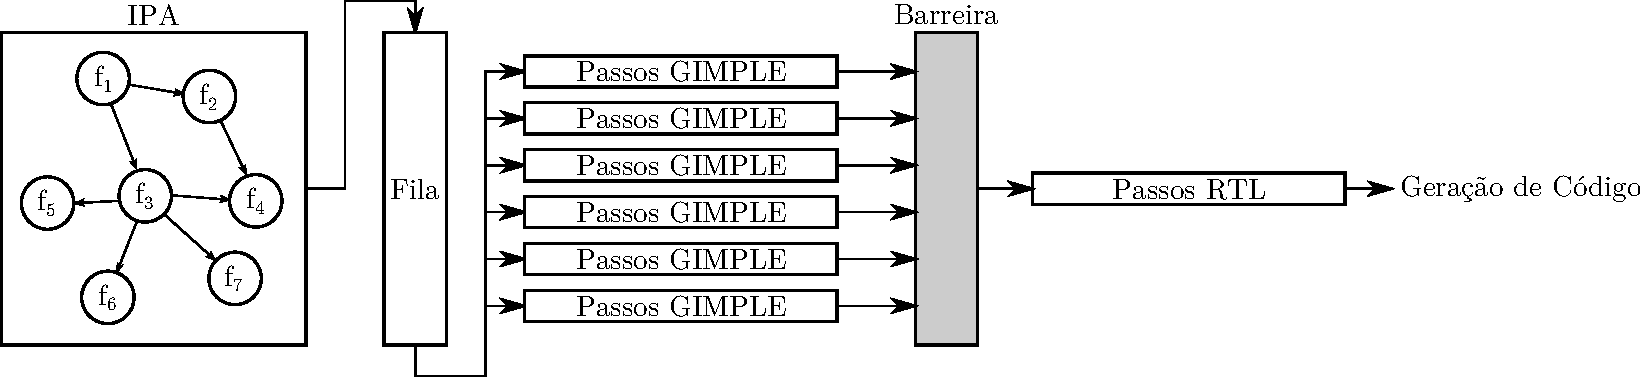
\includegraphics[width=\textwidth]{paralelizacao.pdf}
 \caption{Esquema de paralelização dos passos de otimização.}
 \label{fig:paralelizacao}
\end{figure}
\subsection{Experimentos e Metodologia}

Para validar os resultados obtidos, serão executados dois experimentos:
\begin{enumerate}
    \item Comparação do tempo de compilação do arquivo \texttt{gimple-match.c}
        antes e após a paralelização.


    \item Comparação do tempo total de compilação do GCC antes e após a paralelização.
\end{enumerate}
Tal comparação será realizada utilizando
técnicas de inferência estatística, conforme descrito por
\cite{morettin2017estatistica}: serão
coletadas diversas amostras a respeito do tempo de compilação. Em seguida, será feita alguma suposição a respeito da distribuição
das amostras de acordo com o resultado de um gráfico Q-Q para então calcular um estimador
para o valor esperado e variância. Com isso, serão calculados os intervalos de confiança
sobre a média do tempo de execução para afirmar que ela diminui após a paralelização. Caso
não seja possível encontrar uma distribuição adequada, será utilizado o Teorema do Limite
Central com um número grande de amostras. Em seguida, esse resultado será comparado com o
tempo de compilação utilizando a estrutura LTO, também utilizando as mesmas técnicas estatísticas.

\subsection{Cronograma}

As atividades serão dispostas pelos próximos meses na seguinte forma:

\begin{figure}

  \centering

  \begin{ganttchart}{2019-05}{2020-3}
    \gantttitlecalendar{year,month=shortname} \ganttnewline
    \ganttgroup[progress=0]{Paralelização do GIMPLE}{2019-05}{2019-09} \ganttnewline
    \ganttbar[progress=0]{Separar GIMPLE e RTL}{2019-05}{2019-05} \ganttnewline
    \ganttbar[progress=0]{Remover estados Globais}{2019-05}{2019-07} \ganttnewline
    \ganttbar[progress=0]{Paralelizar o GIMPLE}{2019-07}{2019-09} \ganttnewline
    \ganttmilestone{Experimentos}{2019-09} \ganttnewline
    \ganttgroup[progress=0]{Avaliar a paralelização do RTL e IPA}{2019-10}{2019-12} \ganttnewline
    \ganttgroup[progress=0]{Escrita da Tese}{2019-11}{2020-02} \ganttnewline
    \ganttbar[progress=0]{Escrita do Artigo}{2019-11}{2019-12} \ganttnewline
    \ganttbar[progress=0]{Escrita do Tese}{2019-12}{2020-02} \ganttnewline
    \ganttmilestone{Submissão}{2020-02}
  \end{ganttchart}

  \caption{Cronograma das Atividades.\label{fig:gantt}}
\end{figure}

\begin{itemize}
	\item Separar GIMPLE e RTL: O RTL tem dependências com o \textit{Back End}
	do GCC, sendo assim os passos GIMPLE e RTL serão separados para que seja
	possível paralelizar os passos GIMPLE.

	\item Remover estados globais: O GCC tem muitos estados globais referentes
	aos passos GIMPLE que deverão ser adaptados para a paralelização.

	\item Paralelizar o GIMPLE: Será adicionado código para que os passos do
	GIMPLE executem em paralelo, e em seguida os experimentos serão executados.

	\item Avaliar a paralelização do RTL e IPA: Dependendo do ganho obtido
	na etapa anterior, será avaliado o ganho em paralelizar os passos IPA ou
	o RTL.

    \item Escrita de um Artigo Científico. Tempo destinado a escrita de um
        artigo a respeito dos resultados do trabalho.

	\item Escrita da Dissertação: Tempo destinado a escrita do texto final da
        dissertação.
\end{itemize}
Uma ilustração da distribuição dessas tarefas no tempo está representada na
Figura \ref{fig:gantt}.

\begin{landscape}
%\begin{figure}[ht]
 \vspace*{-2cm}%
 \noindent%
 \hspace*{-2cm}%
    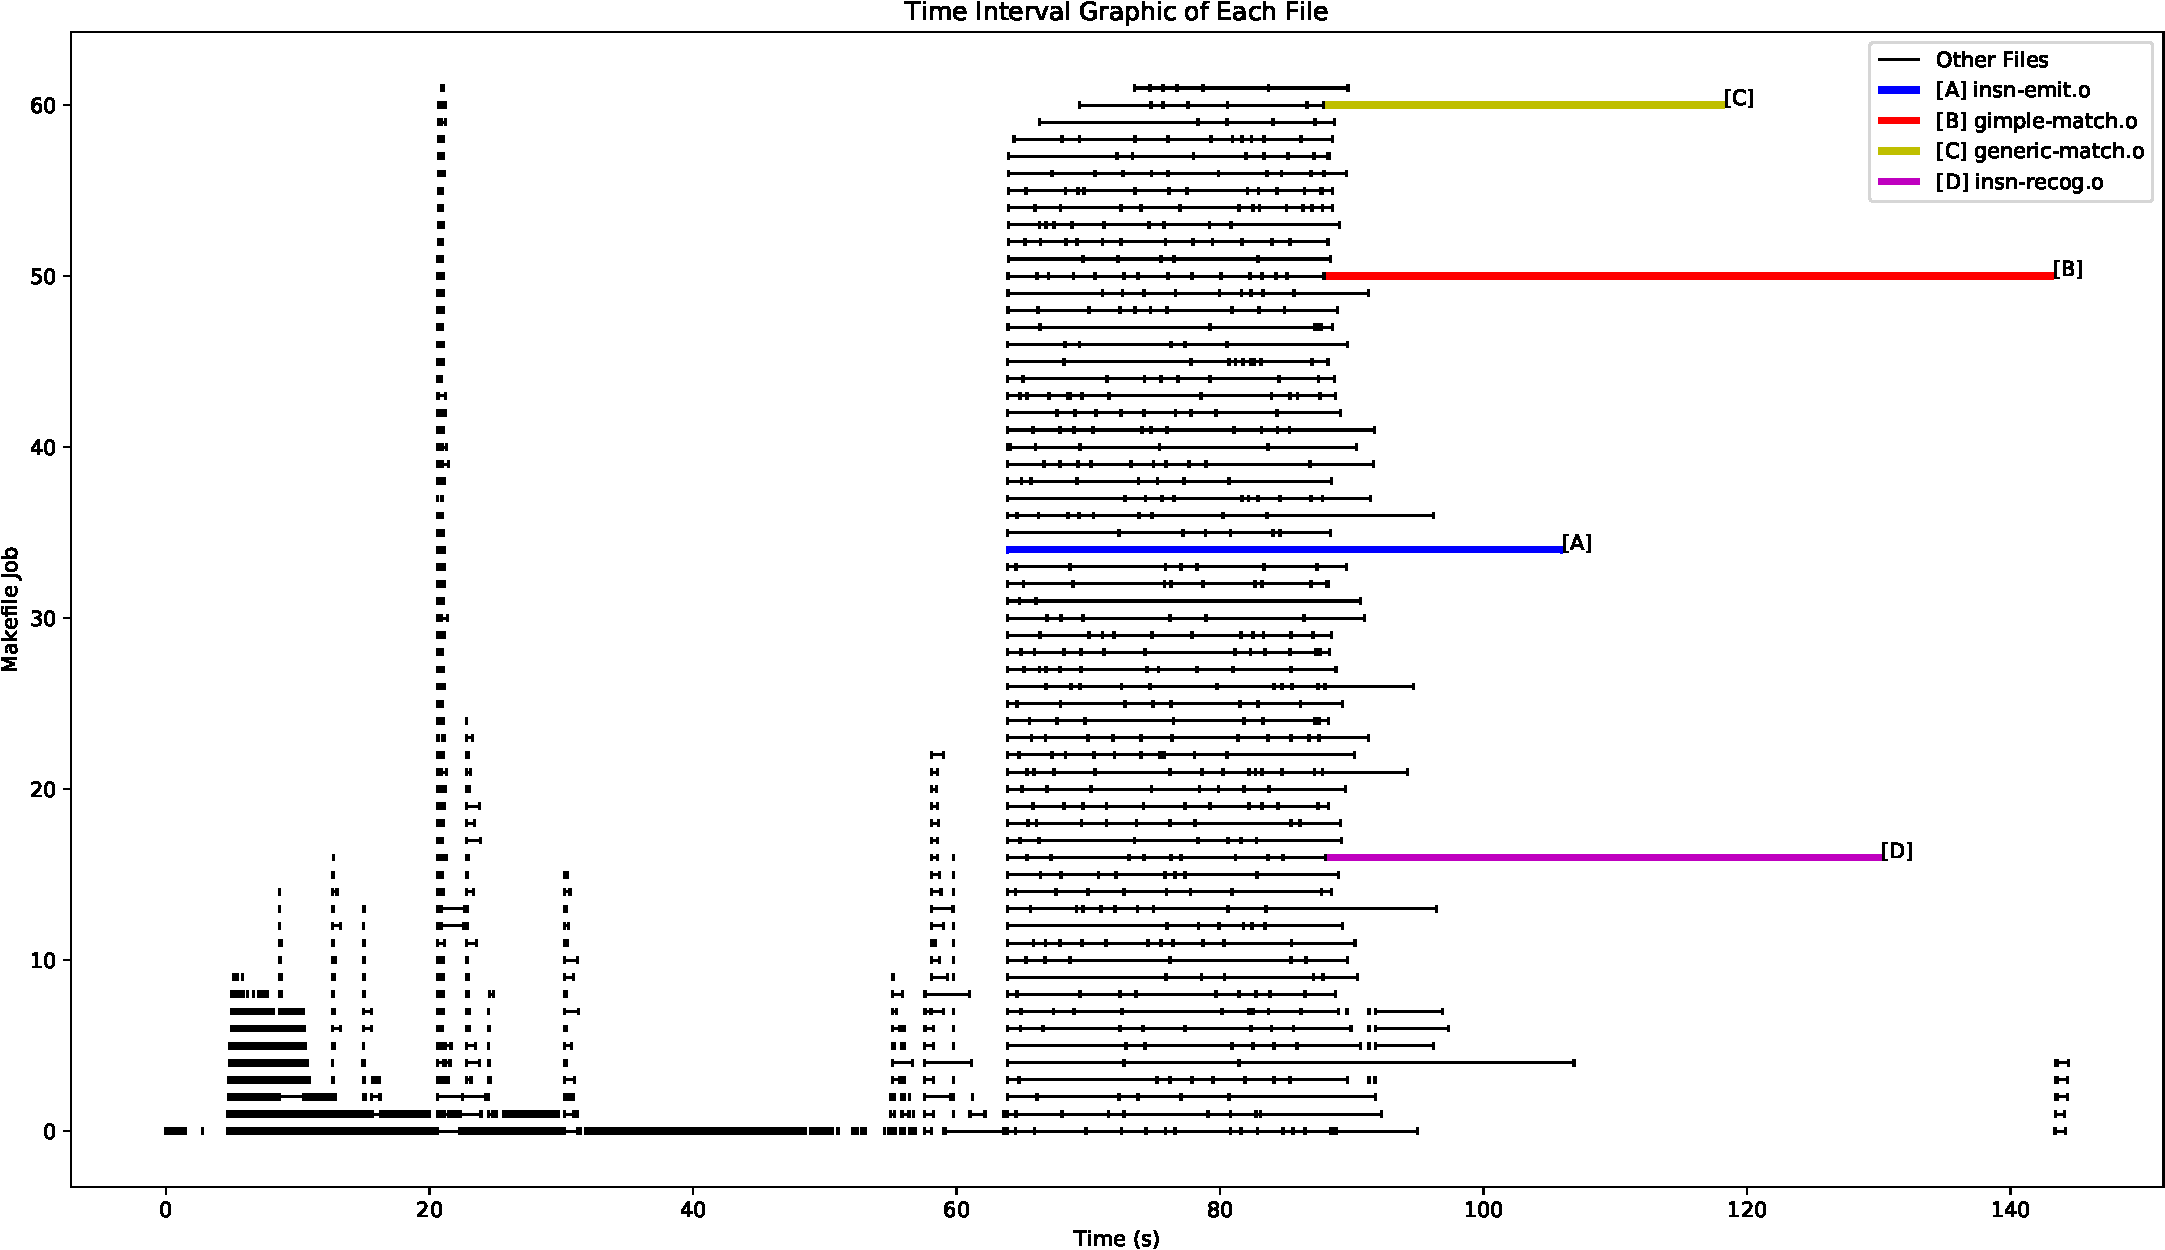
\includegraphics[width=0.9\paperheight]{gcc_timer_classic_crop.pdf}
    \captionof{figure}{Tempo corrido na compilação do GCC em um processador de
    64 núcleos. \textbf{Sem} LTO, sem \textit{Bootstrap}.}
    \label{fig:analysis_classical}
%\end{figure}
\end{landscape}

\begin{landscape}
%\begin{figure}[ht]
 \vspace*{-2cm}%
 \noindent%
 \hspace*{-2cm}%
 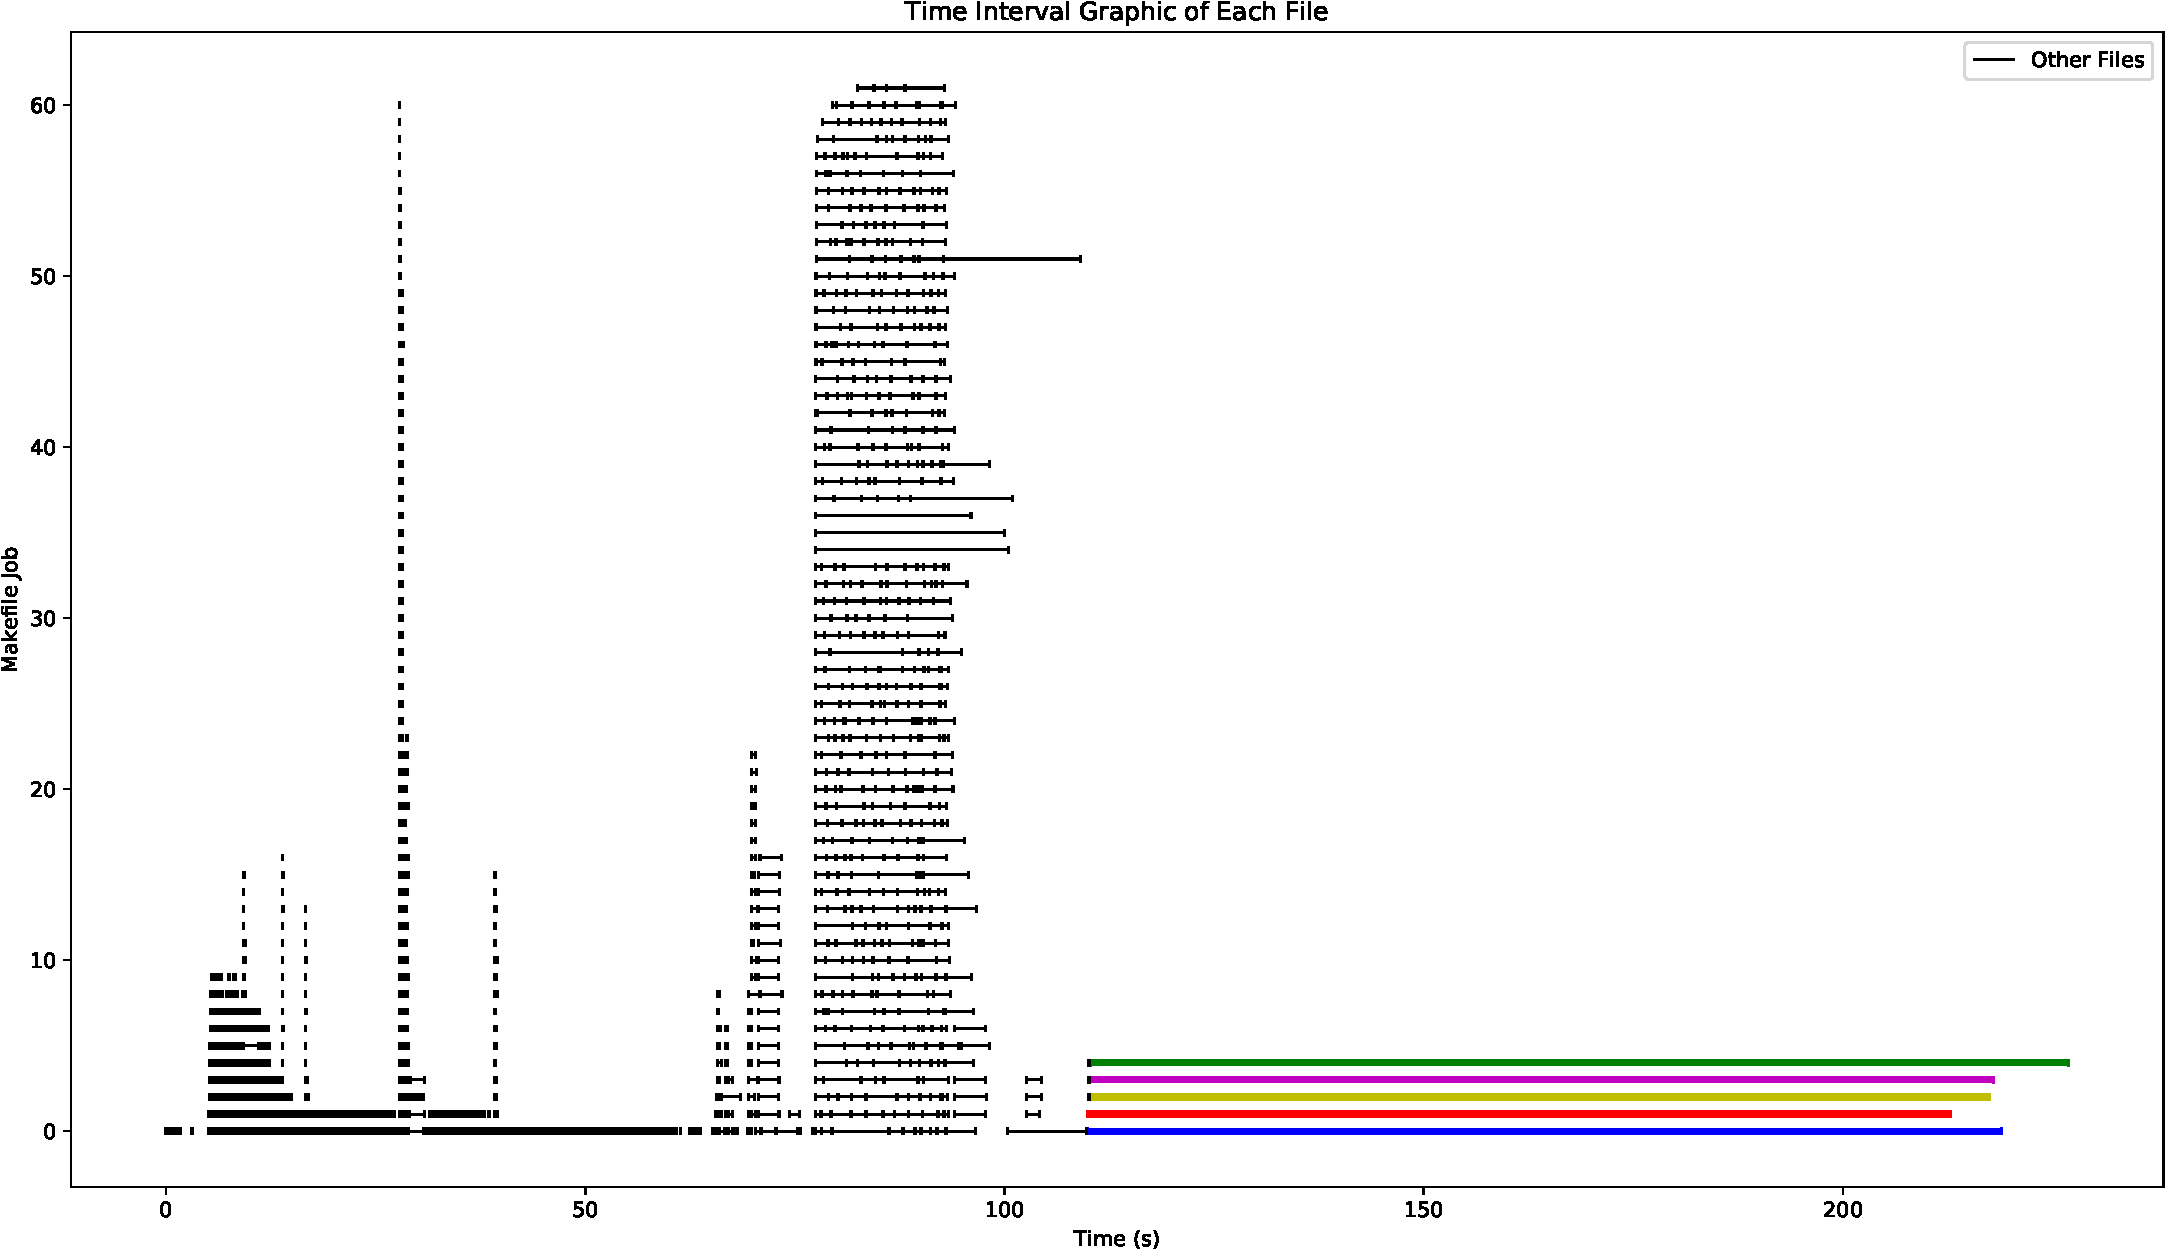
\includegraphics[width=0.9\paperheight]{lto_crop.pdf}
    \captionof{figure}{Tempo corrido na compilação do GCC em um processador de 64 núcleos. \textbf{Com} LTO, sem \textit{Bootstrap}.}
 \label{fig:analysis_lto}
%\end{figure}
\end{landscape}


%%%%%
